\chapter{Workflow}


% ---------------------------------------------------
% USED HARDWARE
\section{Used Hardware\authorA}
For video capturing a \href{https://www.raspberrypi.org/products/raspberry-pi-3-model-b-plus/}{\textit{Raspberry Pi 3B+}} of the Raspberry Pi Foundation with a \href{https://www.raspberrypi.org/products/camera-module-v2/}{\textit{Pi Camera V2}} or a \href{https://www.sainsmart.com/products/wide-angle-fov160-5-megapixel-camera-module-for-raspberry-pi}{\textit{Pi Wide Angle Lens Camera}} are used. The Raspberry Pi sends the video feed to a separate more power full PC over WiFi using a Python3 script \ref{ref:streamPythonScript} since the scripts that are available use \gls{rtsp} (Real Time Streaming Protocol) had a few problems. \newline
For running the DeepTAM a \href{https://support.lenovo.com/us/en/solutions/pd005642}{\textit{Lenovo Think-Station S20}} is used since it requires a dedicated graphics card. Since the DeepTAM is a bit tricky to get it working a \href{https://www.lenovo.com/de/de/laptops/thinkpad/w-series/w550s/}{\textit{Lenovo W550s}} was used as a secondary machine to not loose any progress. For more intense work a server access at the Johannes Kepler University was supplied to work on their system which contains Nvidia Quadro and Nvidia GTX graphics cards. \newline
As the work is based around implementing it on the Audi Autonomous Driving Cup (\gls{aadc}) car a cheaper remote controlled model car was borrowed to test the algorithms in an live environment that is not based on a dataset. The \gls{aadc} car was not used since it has very much power and is pretty expensive.\newline
\begin{figure}[h]
	\centering
	
\includegraphics[height=0.3\textwidth]{./media/images/rpi_logo.eps}
  	\caption{Raspberry Pi Logo\texttrademark
  	\\Src: \url{https://tinyurl.com/njb3a7o}}
  	\label{picamssetup}
\end{figure}

\subsection{Raspberry Pi}
The Raspberry Pi\texttrademark \footnote{Raspberry Pi is a trademark} is running \href{https://www.raspberrypi.org/downloads/raspbian/}{Raspbian Buster} since it is a well optimized version of Debian for the mini computer and only required to be able to execute a Python script to send the raw video feed over http to the the processing device.\newline

\subsection{PC}
The Think-Station and the laptop are running Kubuntu 18.04, which is basically Ubuntu but has a GUI that's a more like Windows and is supported until May 2023. \newline
The Think-Station has a eight core Intel Xeon CPU, a GTX 1660TI and 12GB of RAM inside. \newline
The Laptop has a four core Intel i7 and 8GB of RAM built in.


% ---------------------------------------------------
% USED SOFTWARE
\section{Used Software\authorA}
\textbf{\underline{ADTF}} \newline
At first Ubuntu 16.04 with Automotive Data and Time-Triggered Framework (\gls{adtf}) was used since it's the recommended environment by the \gls{aadc} car manufacturer DigitalWerk. There were many compatibility ans stability issues and it is very difficult to get into the whole system as it's not very beginner friendly. After trying to get the basics of \gls{adtf} working it was clear that switching to ROS might be better. The main problems with \gls{adtf} are, that \gls{adtf} isn't running very stable, requires certain packages to be in a non-standard folders and not having them in the regular location and it is very difficult to work with when using it for the first time.

\textbf{\underline{ROS}} \newline
Running ROS Melodic on Kubuntu 18.04 was pretty straight forward. The instructions on the \href{https://wiki.ros.org/melodic/Installation}{ROS website} \cite{installros} are very clear and can be directly copied without issues. The principle of the workspace is also easy to understand. In the source folder the modules get put in and when compiling the modules automatically generates a setup file to use them. Usage is very easy as the framework already does a lot in the background and using nodes is nearly always setting input and output with a few parameters.

\textbf{\underline{Python}}\footnote{"Python" and the Python logos are trademarks or registered trademarks of the Python Software Foundation} \newline
\href{https://www.python.org}{Python}\cite{PythonHomepage} is a object-oriented, high-level programming language.\emph{\enquote{Its high-level built in data structures, combined with dynamic typing and dynamic binding, make it very attractive for Rapid Application Development, as well as for use as a scripting or glue language to connect existing components together.}}~\cite{WhatIsPython} Next to that the community features a wide range of already written packages which makes it even more simple to create programs.\newline
\begin{figure}[h]
	\centering
	
\includegraphics[width=0.5\textwidth]{./media/images/python_logo.png}
  	\caption{Python Software Foundation logo\texttrademark
  	\\Src: \url{https://tinyurl.com/tfxfbrt}}
  	\label{img:raspiconfig}
\end{figure}


% ---------------------------------------------------
% Setup
\section{Setup\authorA}
As the PC and laptop are not the best idea to run around with, a Raspberry Pi is used instead to stream the video over WiFi to the PC/laptop which are connected to the router over LAN. This makes the camera setup very portable as the pi, camera and powerbank are packed together and only weighs around 500g. The PC can be placed somewhere where and just processing the received video signal.\newline
\begin{figure}[h]
	\centering
	\includegraphics[width=0.8\textwidth]{./media/images/PiSetup.png}
  	\caption{Stream setup with Raspberry Pi, camera and powerbank}
  	\label{picamssetup}
\end{figure}

% ---------------------------------------------------
% SENDING IMAGE FROM RASPBERRY PI TO PC/LAPTOP
\section{Streaming video from Pi to PC\authorA}

\subsection{Enabling Camera}
To use a camera on a Raspberry Pi the camera serial interface (\gls{csi}) needs to be enabled first. This can be done in the built-in tool called \textit{raspi-config}. In this tool as seen in figure \ref{img:raspiconfig} under the subsection called \textit{Interfacing Options} there is a option with the name \textit{Camera}. When the interface is activated a restart is required.\newline
\begin{figure}[h]
	\centering
	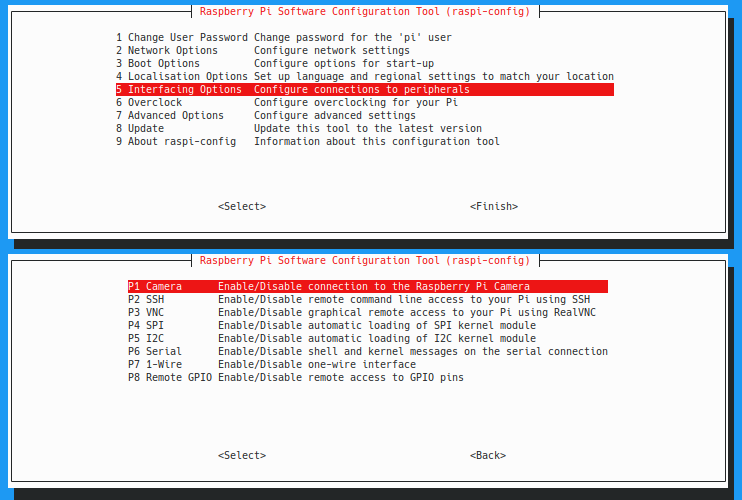
\includegraphics[width=0.9\textwidth]{./media/images/raspiconfig.png}
  	\caption{Activating camerainterface in raspi-config}
  	\label{img:raspiconfig}
\end{figure}

\subsection{Python Script}\label{ref:streamPythonScript}
In listing \ref{code:videostreamMain} at first a \textit{piCamera} instance with the name \textit{cam} is created. As parameters the resolution gets set to \textit{1280x720} pixels and the frame rate is set to \textit{30} frames per second (\gls{fps}). If needed the image can be rotated, e.g the camera is mounted upside down. When starting the camera a output and format are expected. For the output a separate class is used which sets how and when a new frame can be published. The \textit{mjpg} video codec is chosen as a pack for getting MPEG-streams already exists in \gls{ros} and it's not power hungry when running it on the Raspberry Pi as the hardware supports it \cite{raspberrypi3bplusspecs}. \newline
After the camera \enquote{recording} has started successfully the server is started to make the stream accessible to other devices. The server runs until the user closes the script using \textit{CTRL + C}. After closing the server the \textit{finally} block gets called, where the camera \enquote{recording} is stopped so that other programs can use the camera again.\newline
\lstinputlisting[language=Python, firstline=77, lastline=91,caption={Main Function of Camera Feed},label={code:videostreamMain}]{./media/code_snippets/HTTPCamStream.py}

The streamingHandler that is shown in listing \ref{code:videoStreamHandler} handles the actions that are taken when client connects to the Raspberry Pi. At the beginning it checks if the client is requesting the \textit{/stream.mjpg} file. If the client is not requesting that specific file a \textsc{404 Not Found} Error is returned. But if the correct file is requested at first a \textsc{200 OK} code is sent. In addition to the status code headers are send, which tell the client to not use cache. After sending the \textsc{HTTP OK} to the client a permanent loop is started which always waits until a new image from the camera is ready and then sends it to the client as an JPEG image. The loop ensures that the client receives the latest image and such creates a video. Should the client drop the connection an exception is raised which causes the script to drop out of the loop and stops the handler for that specific client until the client connects again.\newline
\lstinputlisting[language=Python, firstline=42, lastline=74, caption={Streaming Handler of CamStream},label={code:videoStreamHandler}]{./media/code_snippets/HTTPCamStream.py}

The behavior when a new image from the pi camera is ready to send is defined in the snipped \ref{code:videoStreamingOutput}. At the beginning it initializes itself with basically no image. \textit{piCamera} class constantly writes into this, as it's defined as the output. When a new image is ready the \textit{picamera} class sends \enquote{\textbackslash xff\textbackslash xd8} as binary data to the output class to notify it. The output class then cuts the buffer so it only contains the current image and sets it in the \textit{frame} variable. To let everybody else know that a new image is ready it sends out a notification.\newline
\lstinputlisting[language=Python, firstline=26, lastline=40, caption={Streaming Output of CamStream},label={code:videoStreamingOutput}]{./media/code_snippets/HTTPCamStream.py}


% ---------------------------------------------------
% RECEIVING IMAGE ON PC/LAPTOP
\section{Receiving images on PC and Laptop\authorA}
For receiving the stream on the PC or Laptop the existing Video-Stream-OpenCV Node is used. Video-Stream-OpenCV is designed to publish videos in the \gls{ros} network which are received from different sources, e.g. USB-cameras, video-files, network cameras and video-streams \cite{videostreamopencv}.

\subsection{MJPG-Stream receiver}
To automate the startup procedure of the node a roslaunch file is used. The lauchfile automatically starts the node and passes the required parameters.\newline
The launchfile shown in \ref{code:mjpgstreamreceiverlaunch} published the received image stream on a topic called \textit{camera}. The video stream provider are the Raspberry Pi's IP-address, port and \textit{/stream.mjpg} directory. 30 \gls{fps} are used since they provide a good balance between amount of traffic and amount of detail in the movement.\newline
\lstinputlisting[language=XML, firstline=3, lastline=14, caption={MJPG-Stream receiver Launch file},label={code:mjpgstreamreceiverlaunch}]{./media/code_snippets/mjpg-stream.launch}


% ---------------------------------------------------
% Cameras
\section{Cameras\authorA}
Nearly every camera has some kind of distortion where the proportions of the image are different to the real world. This is especially noticeable on wide angle lenses which can capture a bigger part of the environment while sitting in the same spot. This can be seen in figure \ref{cameracomparison} that the normal camera only captures a small portion compared to the wide angle lens camera but the wide angle lens creates distortions when getting to the edges.\newline
\begin{figure}[h]
	\centering
	\includegraphics[width=0.8\textwidth]{./media/images/CameraComparison.png}
  	\caption{\textbf{Left Image:} normal Raspberry Pi Camera. \textbf{Right Image:} wide angle lens camera}
  	\label{cameracomparison}
\end{figure}

\subsection{Calibration}
To get rid of the distortions on a wide angle lens camera calibration is needed, which is a mask that gets applied on the image to remove these distortions and rectify it.
For calibration the \textit{camera calibration}-node is used.  Calibration is done by moving and rotating a checkerboard is used since it has good contrast between the tiles and the size of a tile is known and always the same. The node recognizes the checkerboard and calculates the distortion-factors from a series of pictures that have been taken.\newline
The command for starting the node is the following, where amount of tiles, size of tiles in millimeter and camera are set:\newline
\begin{lstlisting}[language=BASH,caption={Start Calibration Node}]
rosrun camera_calibration cameracalibrator.py --size 8x6 --square 0.026 --no-service-check image:=/camera/image_raw camera:=/camera
\end{lstlisting}

This command opens a window which shows the live image feed from the camera and highlights edges on the checkerboard which is shown in figure \ref{img:cameracalibration}. These highlighted edges are points which are used to calculate the distortion parameters using an algorithm that was developed by \href{https://docs.opencv.org/2.4/doc/tutorials/calib3d/camera_calibration/camera_calibration.html}{OpenCV} \cite{cameracalibrationopencv}.\newline
\begin{figure}[h]
	\centering
	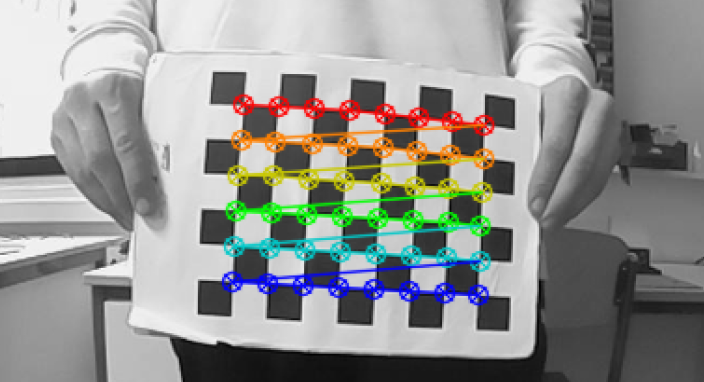
\includegraphics[width=0.8\textwidth]{./media/images/CameraCalibration.png}
  	\caption{Camera calibration}
  	\label{img:cameracalibration}
\end{figure} \newline

When the node has enough reference images the computing of the parameters can start. The duration of the calculations depends on the CPU and how many images have been taken. But most likely it will take around 5 Minutes until the computing is finished. The output data contains two formats of the same data which will look something like shown in figure \ref{code:calibrationyaml}. The output files are normally compatible with all applications without any issues.\newline
\lstinputlisting[language=XML, firstline=1, lastline=14, caption={Calibration file},label={code:calibrationyaml}]{./media/code_snippets/calibration.yaml}


% ---------------------------------------------------
% Things to keep in mind when running ORB-SLAM
\section{Things to keep in mind}\label{ref:orbslamgetgoodresults}
These points are helpful to achieve good results.
\begin{itemize}
    \item \underline{Initialization} \newline
    Avoid movement and too much rotation when the system is initializing.
    
    \item \underline{Rotation} \newline
    Rotation only will not generate any depth information and might even generate wrong points.
    
    \item \underline{Low texture environment} \newline
    Since the ORB-\gls{slam} needs prominent points it won't work properly when there are none or very little points that the algorithm can lock on, e.g. a clear white hallway.
    
    \item \underline{Many/Big moving objects} \newline
    Many or big moving objects generate much data that is not stationary as the algorithm \enquote{thinks} that the vehicle itself is moving.
    
\end{itemize}



% ---------------------------------------------------
% Running Monocular ORB-SLAM2
\section{Running Monocular ORB-SLAM2\authorA}\label{ref:runningmonocularorbslam}
Integrating ORB-SLAM2 \ref{ref:orbslam} is pretty straight forward since there is already \gls{ros} version of it which is very well maintained by \textbf{Lennart Haller} on behav of \textit{appliedAI-Initiative} on \href{https://github.com/appliedAI-Initiative/orb_slam_2_ros}{GitHub} \cite{orbslam2rosgithub}. It just needs to be cloned into the \textit{src} folder of the \gls{ros}-workspace and compiled using the \textit{catkin build} command.When building the packs is finished the generated setup-file has to be sourced. The file is located under \textit{workspace/devel/setup.sh} and can be sourced using the \textit{source setup.sh} command. The \textsc{source}-command is often used to set up variables or commands that are not loaded in the terminal by default. After sourcing the setup all new types of commands that are added by the nodes are available.

\subsection{Calibration file}\label{ref:calibrationorbslam}
Before using the ORB-SLAM the calibration file needs to be created in \textit{src/orb\_slam2/config/config.yaml}. For a baseline the config from another mono-camera can be copied. The calibration part looks like shown in \ref{code:orbslamconfig} and thus the config that the calibration tool generated needs to be converted manually. In the camera\_matrix the values are the following:\newline
\begin{lstlisting}[language=XML,caption={Matrix listing},label={code:calibrationmatrix}]
	  	[camera.fx, 0, camera.cx, 0, camera.fy, camera.cy, 0, 0, 1]
\end{lstlisting}
The distortion\_coefficients need to be mapped like shown in listing \ref{code:calibrationdistortionmatrix}.\newline
\begin{lstlisting}[language=XML,caption={Matrix listing},label={code:calibrationdistortionmatrix}]
	  	[camera.k1, camera.k2, camera.p1, camera.p2, 0]
\end{lstlisting}
Additionally the width, height and \gls{fps} of the incoming video have to be set to use the correct amount of frames and resolution.\newline
\lstinputlisting[language=XML, firstline=3, lastline=17, caption={ORB-SLAM2 config calibration}, label={code:orbslamconfig}]{./media/code_snippets/config.yaml}

\subsection{Launching ORB-SLAM2}
To load the new config file a new launch file is the best way to tell the \gls{slam} to use this config instead of the default parameters. The launch files for ORB-SLAM2 sit in \textit{src/orb\_slam2/ros/launch} where an existing one can be duplicated. The new launch-file should look like the snipped \ref{code:orbslam2launch} except in line \textbf{13} the wrong config is specified. Additionally in the config other settings can be set. For example if the node should publish a pointcloud or position, only do tracking. It is also possible to load an existing map which has been created before and might be used to add additional information or do tracking only on it. When everything is configured it is now possible to launch the ORB-SLAM2 using \textit{roslaunch orb\_slam2\_ros orbslam.launch}. \newline
\lstinputlisting[language=XML,  caption={ORB-SLAM2 launch file}, label={code:orbslam2launch}]{./media/code_snippets/orbslam.launch}

When starting RQt \ref{rqt} and opening the \textsc{Node Graph} it should show, like seen in figure \ref{img:nodegraphstreamorbslam} that the camera-node is sending \textit{image\_raw} to the \textit{orb\_slam2\_mono}-node. If that is not the case it is most likely due to some spelling error or a \textit{remap} line in the launch-file of the ORB-SLAM2.\newline
\begin{figure}[h]
	\centering
	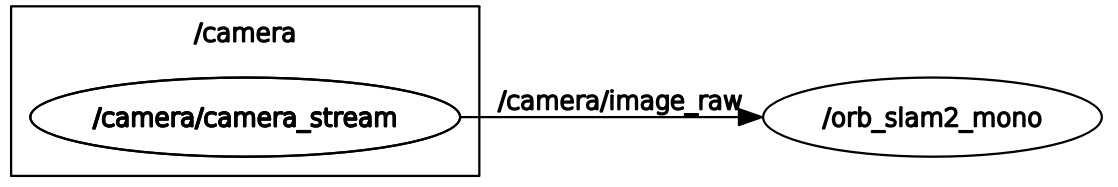
\includegraphics[width=0.8\textwidth]{./media/images/nodegraphstreamorbslam.png}
  	\caption{Node Graph with Stream and ORB-SLAM}
  	\label{img:nodegraphstreamorbslam}
\end{figure}


% ---------------------------------------------------
% Running Stereo ORB-SLAM2
\section{Running Stereo ORB-SLAM2\authorA}
As explained in the ORB-SLAM chapter \ref{ref:orbslam} there are some problems with running it with a single-camera setup. The main problem is that on a monocular image the scale information is not provided an thus drifting occurs. A way to bypass this problem is by using two cameras looking in the same direction but with a slight offset. The setup with two cameras then works a bit more like eyes where the depth perception is easier when having both eyes open compared to only having one open.

\subsection{Hardware setup}
Since stereo cameras and synchronization boards are not cheap, two identical Raspberry Pi's with the same camera are used for the testing environment. The two Raspberry Pi's have the same SD card type, operating system and packages to prevent any timing difference as much as possible. There are solutions that use a special board with a circuit for synchronizing the cameras or even boards that already have two cameras mounted. The problem is that they are pretty expensive. The Cameras are taped on a stick of wood with a distance of around six centimeters to mimic the average distance between the human eyes.

\subsection{Calibration}
Calibration in this testing environment is pretty straight forward as the cameras used are the normal Pi Cameras v2 which basically have nearly no distortion. Just for being on the save side calibration was done on both cameras and the values only are slightly different. So the format that was entered in the config was the same as on the monocular \gls{slam} calibration \ref{ref:calibrationorbslam}. If cameras with distortion are used there are more values that are required a bit further down in the config.

\subsection{Software setup}
The same Python script as already explained in section \ref{ref:streamPythonScript} is used on both devices to make the camera feed available on the local network. To receive these streams two MJPG-Stream receivers are required. Note that the camera name must be unique, e.g they may be named \textsc{lcamera} \ref{code:leftcameralaunch} and \textsc{rcamera} \ref{code:rightcameralaunch} to know which is the left and right camera. Also required is to set the stream receiver to the correct IP-address since it is important later. Re-building isn't necessary since only the config and launchfile change, which are not compiled but instead loaded every time the \gls{slam} starts.\newline
\begin{lstlisting}[language=XML,caption={Left camera stream launch file},label={code:leftcameralaunch}]
	  	<arg name="camera_name" value="lcamera" />
\end{lstlisting}
\begin{lstlisting}[language=XML,caption={Right camera stream launch file},label={code:rightcameralaunch}]
	  	<arg name="camera_name" value="rcamera" />
\end{lstlisting}

Since the two video streams are still on a topic that the \gls{slam} doesn't subscribe on it is necessary to remap the two streams to the correct topics. This can be done in a launchfile for the stereo ORB-SLAM.
To do this it is only required to add two lines which are shown in listing \ref{code:stereoorbremap} at line \textbf{5} and \textbf{6} before all other settings for the \gls{slam} get set. This remaps the nodes that triesw to subscribe to e.g \textit{/image\_right/image\_color\_rect} to the correct topic that is publishing the image named \textit{/rcamera/image\_raw} \newline
\lstinputlisting[language=XML, caption={ORB-SLAM2 stereo launch file}, label={code:stereoorbremap}]{./media/code_snippets/orbslamstereo.launch}

\subsection{Launching}
When starting the stereoscopic launch for the \gls{slam} using the command \ref{cmd:stereoorbslamlaunch} ,it should indicate in RQt \ref{rqt} that the ORB-SLAM subscribed onto both video streams like shown in figure \ref{img:nodegraphstereoslam}. If only one is connected it might be caused by a misspelled word in the remap line or when naming the cameras in the stream launch file. Additionally when opening the \textit{Image View} and selecting \textsc{/orb\_slam2\_stereo/image\_image} as the source the image of the left camera should be displayed.\newline
\begin{lstlisting}[language=bash, label={cmd:stereoorbslamlaunch}]
    roslaunch orb_slam2_ros stereo-slam.launch
\end{lstlisting}
\begin{figure}[h]
	\centering
	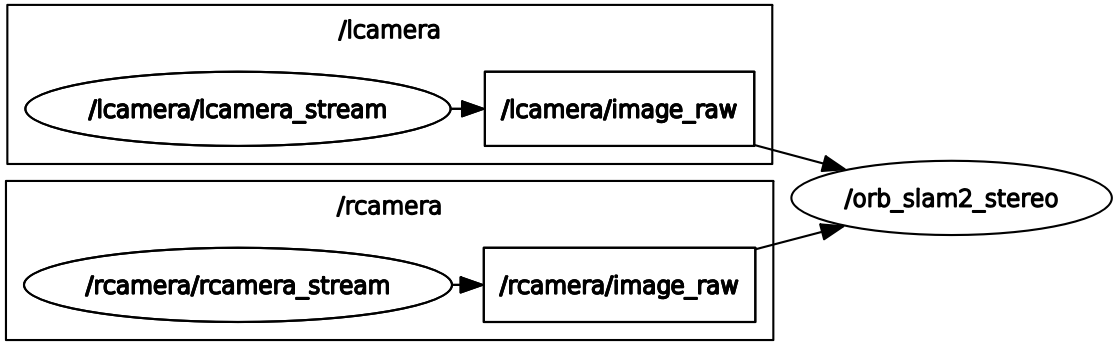
\includegraphics[width=0.8\textwidth]{./media/images/nodegraphstereoorbslam.png}
  	\caption{Node Graph with Stereo ORB-SLAM2}
  	\label{img:nodegraphstereoslam}
\end{figure}
Note that the \gls{slam} will freak out when the cameras are not \enquote{looking} at the same picture or are at different angles.

% ---------------------------------------------------
% Results
\section{Result with ORB-SLAM}
The result when running the ORB-\gls{slam} is a 3D map that consist of many dots that are at specific points in a space. To get the map out of the \gls{ros} node it is necessary to call a service \ref{ref:rosservice}. Depending on the used camera type the command looks like one shown in listing \ref{code:saveorbslammap}.\newline
\begin{lstlisting}[language=BASH,caption={Saving map from ORB-SLAM},label={code:saveorbslammap}]
rosservice call /orb_slam2_rgbd/save_map map.bin
rosservice call /orb_slam2_stereo/save_map map.bin
rosservice call /orb_slam2_mono/save_map map.bin
\end{lstlisting}
When viewing the map in a programm like RViz \ref{rviz} it should look similarly to figure \ref{img:orbslammaptopdown} \newline.
\begin{figure}[h]
	\centering
	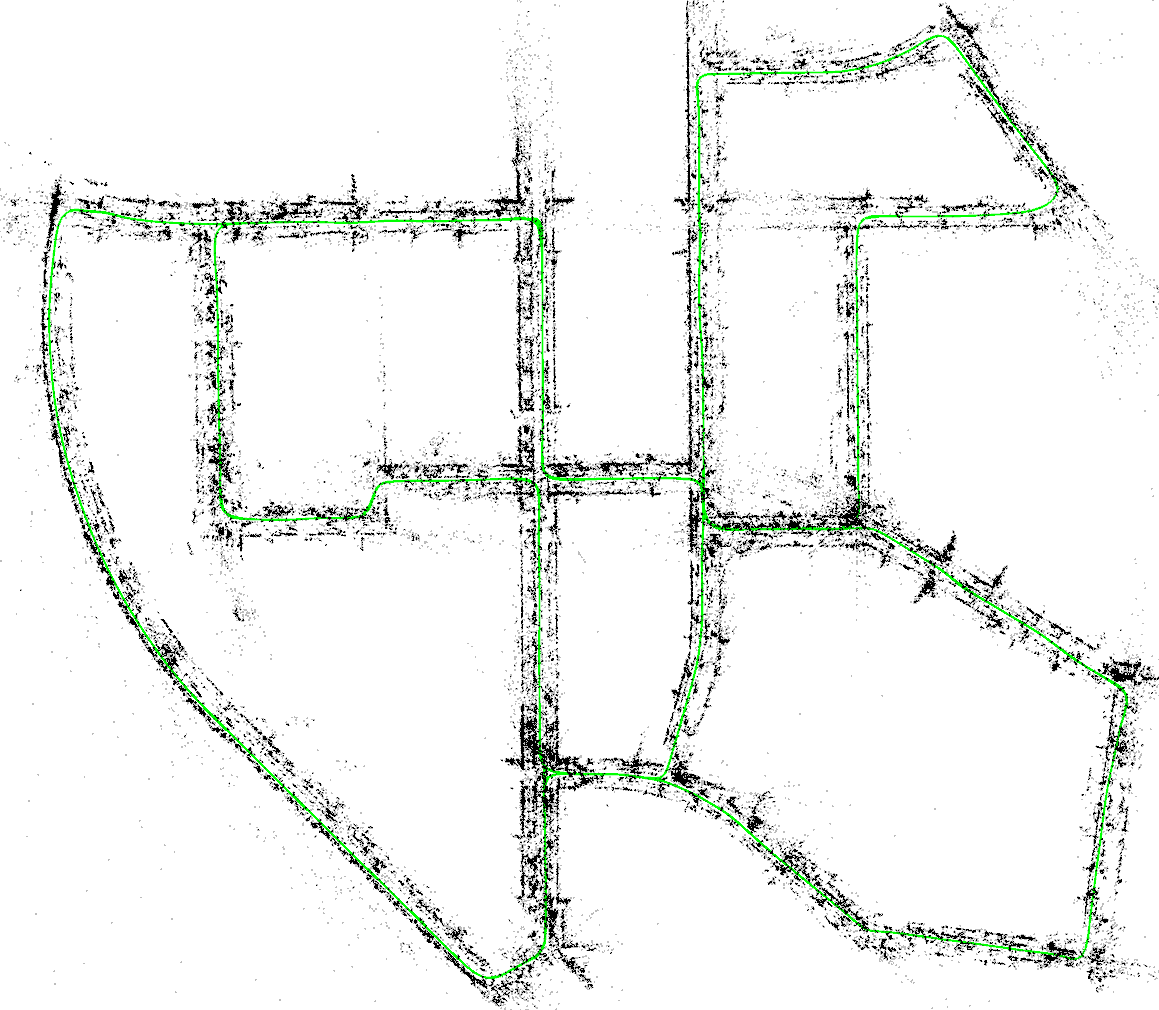
\includegraphics[height=0.5\textwidth]{./media/images/orbslamtopdown.png}
  	\caption{ORB-SLAM Top Down
  	\\ Src: \url{https://tinyurl.com/swoouaa}}
  	\label{img:orbslammaptopdown}
\end{figure}


% ---------------------------------------------------
% Running LSD-SLAM
\section{Running LSD-SLAM\authorA}
Running the LSD-SLAM is not as straight forward as it is on the ORB-SLAM \ref{ref:runningmonocularorbslam}. The implementation of the LSD-SLAM is made to use it with \gls{ros} out of the box but the \href{https://github.com/tum-vision/lsd_slam}{original version} \cite{githublsdslamtum} by the Computer Vision Group at the Technical University of Munich was not updated in the past 5 years and such had some problems when running it on a newer version of \gls{ros} and Ubuntu. Therefor an more up-to-date version by Kevin George was used where he added support for newer versions of libraries and fixed some bugs. Even though the \href{https://github.com/kevin-george/lsd_slam}{fork by Kevin George} \cite{kevingeorgelsdslam} was updated 2 Years ago there were still some bugs and other problems. So a fork was created with the fixes to address the problems that where in Kevin George's Repository. The fork includes bug fixes to run LSD-SLAM on \gls{ros}-Melodic and Ubuntu 18.04 pretty much out of the box.\newline
The \href{https://github.com/MrMinemeet/lsd_slam}{new fork} \cite{alexandervoglspergerlsdslam} contains implementation to use \textsc{Eigen v3.2.5} that doesn't need to be installed, a special version of General Graph Optimization (\gls{g2o}) and a \textsc{CSPARSE}-directory path fix.\newline

% Listing of errors when building LSD-SLAM from original source
\subsection{Errors when building from source original source}
This list shows typical errors when building the LSD-SLAM from source and how to fix or at least bypass them.

%Cannot bind non_const lvalue to rvalu
\subsubsection{Cannot bind non\_const lvalue to rvalue}
When receiving an error like shown in listing \ref{error:non_const_lvalue_to_rvalue} this is most likely due to a datatype error where the functions expects a \textsc{double} but a \textsc{float} is defined.
to fix this, it is only necessary to change \textit{float x,y,z;} to \textit{double x,y,z;} in the two files in the error.\newline
\begin{lstlisting}[language=bash,label={error:non_const_lvalue_to_rvalue}]
PointCloudViewer.h:136:26: error: cannot bind non-const lvalue reference of type 'qreal& {aka double&}' to an rvalue of type 'qreal {aka double}'
   frame.getPosition(x,y,z);
   
PointCloudViewer.cpp:327:44: error: cannot bind non-const lvalue reference of type 'qreal& {aka double&}' to an rvalue of type 'qreal {aka double}'
        camera()->frame()->getPosition(x,y,z);
\end{lstlisting}

% no such function found: g2o::OptimizationAlgorithmLevenberg
% base_vertex.h not found
\subsubsection{\textit{no such function found: g2o::OptimizationAlgorithmLevenberg} and \textit{base\_vertex.h not found}}
This error occurs due to a change in newer \gls{g2o} versions. To fix this, it is required to install the \textit{g2o c++03} version. The fix  itself for this error can be found at \gls{g2o} \ref{ref:g2o}.

% cannot find -lcparse
\subsubsection{/usr/bin/ld: cannot find -lcsparse}
The error shown in \ref{error:cannotfindlcsparse} most likely accuress when catkin is looking for files that are in a different folder that expected by it.\newline
\begin{lstlisting}[language=bash,label={error:cannotfindlcsparse}]
[ 91%] Linking CXX shared library /home/alex/lsd-slam_ws/devel/lib/liblsdslam.so
/usr/bin/ld: cannot find -lcsparse
collect2: error: ld returned 1 exit status
\end{lstlisting}
To fix it the paths where the required files are, have to be included in the \textit{CMakeList.txt} file which can be found in the source folder. Add the block shown in \ref{code:csparseincludedir} at the top of the file and replace \textsc{csparse} and \textsc{cxsparse} with \textsc{\$\{CSPARSE\_INCLUDE\_DIR\}} at the line where \textit{target\_link\_libraries} is adding the links to libraries.\newline
\begin{lstlisting}[label={error:csparseincludedir}]
find_path(CSPARSE_INCLUDE_DIR NAMES cs.h
  PATHS
  /usr/include/suitesparse
  /usr/include
  /opt/local/include
  /usr/local/include
  /sw/include
  /usr/include/ufsparse
  /opt/local/include/ufsparse
  /usr/local/include/ufsparse
  /sw/include/ufsparse
  PATH_SUFFIXES
  suitesparse
  )
\end{lstlisting}

% liblsdslam.so: Warning: undefined reference »..«
\subsubsection{liblsdslam.so: Warning: undefined reference »..«}
This error is a batch of errors that occur at the same time.
It is mainly that references cannot be found by the system. The error might look something like shown below and is very easy to fix. The problem is that the \textit{libsuitesparse-dev} package is missing. When installing the package and then compiling \gls{g2o} it should work again.\newline
\begin{lstlisting}[language=bash]
.../liblsdslam.so: Warning: undefined reference cs_di_post
.../liblsdslam.so: Warning: undefined reference cs_di_etree
.../liblsdslam.so: Warning: undefined reference cs_di_sfree
\end{lstlisting}

% double free or corruption
\subsubsection{double free or corruption}
\begin{lstlisting}[language=bash]
double free or corruption (out)
Aborted (core dumped)
\end{lstlisting}
The error shown in listing is due to changes in newer versions of Eigen. To fix this the easiest way is to download the version \textsc{3.2.5} from the \href{https://bitbucket.org/eigen/eigen/downloads/?tab=tags}{Eigen Bitbucket website} \cite{eigenbitbucket} and un-compress it somewhere where it can stay during the build process.
In the \textit{CMakeList.txt} of the \textit{lsd\_slam\_core} add the code like shown in listing \ref{code:lsdcorecmakelist} and replace \textsc{PATH} with the just unpacked folder path.\newline
\begin{lstlisting}[language=bash, label={code:lsdcorecmakelist}, caption={CMakeList in lsd\_slam\_core with fix for Eigen}]
set(EIGEN3_INCLUDE_DIR "PATH")
include_directories(
  include
  ${EIGEN3_INCLUDE_DIR}
\end{lstlisting}

% g2oTypeSim3Sophus.h Errors
\subsubsection{g2oTypeSim3Sophus.h Errors}
Another error that likes to come up multiple times in the same file. 
These errors will look something like show below but in a much bigger scale.\newline
\begin{lstlisting}[language=bash]
lsd_slam/lsd_slam_core/src/GlobalMapping/g2oTypeSim3Sophus.h:96:33: error: template argument 1 is invalid
   Eigen::Map<const g2o::Vector7d> v(m);
\end{lstlisting}
This error occurs because of some changed in \textsc{Eigen} and is a relativly easy fix.
To fix it it is only necessary to change the code show below from \textit{line 1} to \textit{line 2} in the \textit{g2oTypeSim3Sophus.h} \cite{g2oTypeSim3Sophus.hfix}.\newline
\begin{lstlisting}[language=C++, caption={Fix for g2oTypeSim3Sophus.h}]
Eigen::Map<const g2o::Vector7d> v(m);
Eigen::Map<const Eigen::Matrix<double, 7 ,1>> v(m);
\end{lstlisting}


% Could not find package configuration file provided by "Eigen"
\subsubsection{Couldn not find package configuration file provided by \textsc{Eigen}}
When receiving a error message that states something similiar to the message below it is most likely because of a naming difference in the \textit{CMakeList.txt}.\newline
\begin{lstlisting}[language=bash]
lsd_slam/lsd_slam_viewer/CMakeLists.txt:30 (find_package):
  By not providing "FindEigen.cmake" in CMAKE_MODULE_PATH this project has
  asked CMake to find a package configuration file provided by "Eigen", but
  CMake did not find one.
\end{lstlisting}
The fix is to rename \textit{Eigen} to \textit{Eigen3} in the \textit{CMakeList.txt} in the stated path.


% g2o No matching function for call
\subsubsection{g2o No matching function for call}
When getting this error it is because of a non-compatible version of \gls{g2o}. To fix this it is required to uninstall all other versions of \gls{g2o} and then install a working version like explained at \ref{ref:g2o}.

% ros/ros.h: No such file or directory
\subsubsection{ros/ros.h: No such file or directory}
If an error message like shown occurs it is because the catkin directories are not included by default.\newline
\begin{lstlisting}[language=bash]
lsd_slam/lsd_slam_core/src/IOWrapper/ROS/ROSImageStreamThread.h:27:10: fatal error: ros/ros.h: No such file or directory
\end{lstlisting}
To fix it it is required to add \textit{\${catkin\_INCLUDE\_DIRS}} to the \textit{include\_directories} in the CMakeList-File \cite{rosroshnosuchfileordirectory}. It should look like the listing below afterwards.\newline
\begin{lstlisting}[language=C++, caption={Fix for ros/ros.h: No such file or directory}]
include_directories(
  include
  ${EIGEN3_INCLUDE_DIR}
  ${PROJECT_SOURCE_DIR}/src
  ${PROJECT_SOURCE_DIR}/thirdparty/Sophus
  ${CSPARSE_INCLUDE_DIR} #Has been set by SuiteParse
  ${CHOLMOD_INCLUDE_DIR} #Has been set by SuiteParse
  ${OpenCV_INCLUDE_DIRS}
  ${catkin_INCLUDE_DIRS}
)
\end{lstlisting}


% ‘CV_GRAY2RGB’ & ‘CV_RGB2GRAY’ not declared
\subsubsection{CV\_GRAY2RGB \& CV\_RGB2GRAY not declared}
If the following error comes up it is due to a change in the naming scheme.\newline
\begin{lstlisting}[language=bash]
error: 'CV_GRAY2RGB' was not declared in this scope
   cv::cvtColor(keyFrameImage8u, res, CV_GRAY2RGB);
\end{lstlisting}
The fix is just to replace \textit{cv\_} with \textit{vc::COLOR\_} and should look like e.g.  \newline
\begin{lstlisting}[language=C++, caption={Example fix for \'CV\_GRAY2RGB\' \& \'CV\_RGB2GRAY\' not declared}]
cv::COLOR_GRAY2RGB
\end{lstlisting}

% Installing LSD-SLAM with fixed repository
\subsection{Installing LSD-SLAM from fixed repository}
To run the LSD-SLAM a few packages are required. They can be installed using\newline
\begin{lstlisting}[language=bash, caption={Installing prerequisites for LSD-SLAM}]
    apt install ros-melodic-cv-bridge liblapack-dev libblas-dev freeglut3-dev libqglviewer-dev-qt4 libsuitesparse-dev libx11-dev
\end{lstlisting}

and then creating a link for \textit{libQGLViewer} to the file the LSD-SLAM is looking for. To create the softlink this command is used wich basically creates a link just without the \textsc{-qt4} at the end.\newline
\begin{lstlisting}[language=bash,caption={Creating softlink for libQGLViewer.so}]
    sudo ln -s /usr/lib/x86\_64-linux-gnu/libQGLViewer-qt4.so /usr/lib/x86\_64-linux-gnu/libQGLViewer.so
\end{lstlisting}

\subsubsection{G2O}\label{ref:g2o}
As the LSD-SLAM requires a special version of the \gls{g2o} framework all other versions that have been installed on \gls{ros} need to be removed completely. For this first the \textit{ros-melodic-g2o} package needs to be purged and the leftovers need to be deleted to not conflict with the special version that is going to be installed later using.\newline
\begin{lstlisting}[language=bash, caption={Removing leftover from \gls{g2o}}]
    rm -r /usr/local/lib/libg2o* /usr/local/include/g2o /usr/local/lib/g2o /usr/local/bin/g2o*
\end{lstlisting}

To install the correct version of \gls{g2o} it needs to be cloned from \href{https://github.com/felixendres/g2o.git}{GitHub} \cite{g2ofelixendres} which creates a g2o folder in which a \textit{build}-folder has to be created. In the \textit{build} folder two commands have to be executed in order to install the framework.\newline
\begin{lstlisting}[language=bash]
    cmake ..
    sudo make install
\end{lstlisting}

\subsubsection{Eigen}\label{ref:eigen}
When done it is also necessary to download a specific version of the \textsc{Eigen}-library which has to be in a location where it is not likely to be moved as the full path is required. The Path should look a bit like this \textit{/home/alex/Projects/LSD-SLAM/eigen-eigen-bdd17ee3b1b3/}. This path needs to be set in the \textit{CMakeList.txt} in the \textit{lsd\_slam\_core} folder which was contained in the LSD-SLAM repository. In the file at line \textbf{106} there should be a placeholder like shown in \ref{code:eigenpathdir}, which has to be replaced with the path of \textsc{Eigen}.\newline
\lstinputlisting[language=XML, firstline=106, lastline=106, caption={CMakeList Eigen Directory}, label={code:eigenpathdir}]{./media/code_snippets/LSD-SLAM-Core-CMakeList.txt}

\subsubsection{Building LSD-SLAM}\label{ref:buildinglsdslam}
When these steps are done there is only one last command to be executed in the root directory of the workspace. To compile the LSD-SLAM in the \textit{src} folder the command is \newline
\begin{lstlisting}[language=bash]
    catkin_make
\end{lstlisting}
which may take some time. 


\subsection{Things to keep in mind}\label{ref:lsdslamgetgoodresults}
These points are helpful to get good results and some to keep in mind when running the \gls{slam}. \cite{githublsdslamtum}.
\begin{itemize}
    \item \underline{Resolution} \newline
    A recommended resolution for the video input is \textsc{640x480} pixel. Higher resolutions are possible but require more computing power and changes in hard-coded values.
    
    \item \underline{Framerate} \newline
    At least 30 \gls{fps} or more should be delivered to the \gls{slam} to get good results when moving.
    
    \item \underline{Global shutter} \newline
    The camera should have a global shutter where the the image is taken all at once. Rolling shutters which scan the image from top to bottom \cite{globalrollingshutter}. This might lead to changes while the scan is running and thus generating false information. This wrong information then leads to inferior results.
    
    \item \underline{Field of View} \newline
    A camera lens that has a wide field of view (\gls{fov}) is recommended to get a bigger area that the camera can capture and thus is able to fetch more information. A lens with \textsc{130\degree} or more is recommended.
    
    \item \underline{Camera Movement} \newline
    It is a very important aspect. Typically the LSD-\gls{slam} is designed to move more sideways but when having a wide \gls{fov} it is also possible to have forwards and backwards motion.
    Rotating the camera without moving it will not work since there is not enough camera translation. 
    
    \item \underline{Different results when running multiple times} \newline
    Since the LSD-\gls{slam} is designed to be non-deterministic the results will not be the same all the time. E.g when running a dataset the map will most likely be similar but not exactly the same. This is due to parallelisation and some slight changes in keyframe which have a big impact on everything that follows in the processing order and thus creates different results.
    
\end{itemize}



% ---------------------------------------------------
% DeepTAM
\section{DeepTAM\authorB}
In the following section the process of getting DeepTAM to run will be explained. Also the Problems of our workflow will be listed.

\subsection{Ubuntu 16.04}

The first attempt was to work with Ubuntu 16.04 and Python3, following the instructions given by Uni-Freiburg. At first a virtual environment manager needed to be installed with pip3(a package manager for Python3). Here pew is used and installed. Afterwards a new environment is created and entered. These are the commands:  

\begin{lstlisting}[language=bash]
    pip3 install pew
    pew new deeptam
    pew in deeptam
\end{lstlisting}

The next step was to install tensorflow(\gls{tf}), minieigen and scikit-image, also with pip3. Here the first error occurred. The error is that during the installation of minieigen Eigen/Core cannot be found. This problem can be worked around with the following commands.

\begin{lstlisting}[language=bash]
    sudo apt-get install libeigen3-dev
    sudo apt-get install python3-minieigen 
    sudo apt-get install libboost-all-dev
\end{lstlisting}

After these commands minieigen can be installed with pip3. The next step is to clone and build lmbspecialops. lmbspecialops is a collection of tensorflow ops. The ops focus on networks for predicting depth and camera motion but can also be useful for other tasks. 
